\documentclass{sigish}
\begin{document}

% ------ Enter task number (1-3) here
\def\taskno{3}

% ------ Enter your group letter here
\def\groupno{D}

% ------ Enter your group size here
\numberofauthors{4}

% ------ Enter details for each group member here
\author{
% 1st. group member
\alignauthor J{\"u}rgen Ratzenb{\"o}ck\\
       \affaddr{Mat.nr.: 1256030}\\
       \email{juergen.ratzenboeck@gmail.com}\\ % or whichever you prefer
       \affaddr{Score Percentage: 25\%}\\ % adapt accordingly
% 2nd. group member
\alignauthor Jonathan-Edwin Asamoah\\
       \affaddr{Mat.nr.: 1457554}\\
       \email{asamoahjonathan@outlook.com}\\
       \affaddr{Score Percentage: 25\%}\\
\and
% 3rd. group member
\alignauthor Mhd Mousa Hamad\\
       \affaddr{Mat.nr.: 1556686}\\
       \email{mhd.mousa.hamad@gmail.com}\\
       \affaddr{Score Percentage: 25\%}\\
% 4th. group member
\alignauthor  Luka Vukas\\
       \affaddr{Mat.nr.: 1557457}\\
       \email{vukaslukaa@gmail.com}\\
       \affaddr{Score Percentage: 25\%}\\
}

% leave untouched!
\title{Learning from User-generated Data SS2016 -- Task \taskno}
\subtitle{Group \groupno}
\maketitle


% The following is just an example structure. Change to whatever works best for you. 
% However, make sure to include everything requested in the exercise description.

\section{Description of Task \taskno}

In this task, we should predict a set of movie ratings for 200.000 (user, movie) tuples. To fulfill the task, four different datasets are provided. The first one contains 800.000 (user, movie, rating) triples which represent previous movie ratings. The second one contains more details about the movies namely, title, release year and genres. The third one contains some information about the users who rated the movies namely, gender, age range, job and zip-code. The data provided by these three files combined with extended information crawled from multiple on-line movie sources should be used in experimenting and evaluating different hybrid recommendation systems. The fourth file contains a set of (user, movie) tuples which should finally be enriched by predicted user ratings for the movies using the best evaluated recommendation system.

The remainder of this paper is organized as follows. In section 2 we provide an overview and a short analysis on the provided datasets. Section 3 explains how we addressed this task. It also proposes our parallelized and monolithic approaches to predict the missing ratings. Section 4 presents how we tested our approaches using different configurations and also the setups conducted for these configurations. Section 5 shows the results for different setups, and the last section wraps up the task by concluding it.

\section{Data Analysis}

Data analysis was performed mainly in tasks 1 and 2. The first file of this task contains 800167 (user\_id, movie\_id, rating) tuples used for training with the highest rating density at a four. The second file of this task contains 200042 (user\_id, movie\_id) tuples used for predicting the final ratings with 25 new movie\_ids which don't exist in the training set.

The second file contains 3883 (id, title, genres) triples which equal the number of total movies to be rated by the users. Three different on-line movie sources were crawled to gather additional information about the movies (OMDB, TMDB, DBPedia). We were able to enrich (94\%, 92\%, 82\%) of the movies with external information from (OMDB, TMDB, DBPedia) respectively.

OMDB was used as the main information source, where TMDB and DBPedia were used to enrich this source either by filling in the missing values or by extending the basic information. This process led to 95 features for each movie, which were analyzed and processed to end up with 17 important features that have relatively high densities.

The third file provided contains 6040 (id, gender, age, job, zip-code) quintuples which also fits the number of users who occur in the user-movie datasets for the ratings. The user information provided was complete and sound (no missing or unknown values). Figure \ref{fig:agerangegender} shows that users tend to be males (71\%) and in the age range of [25, 34] (34\%).

\begin{figure}
\centering
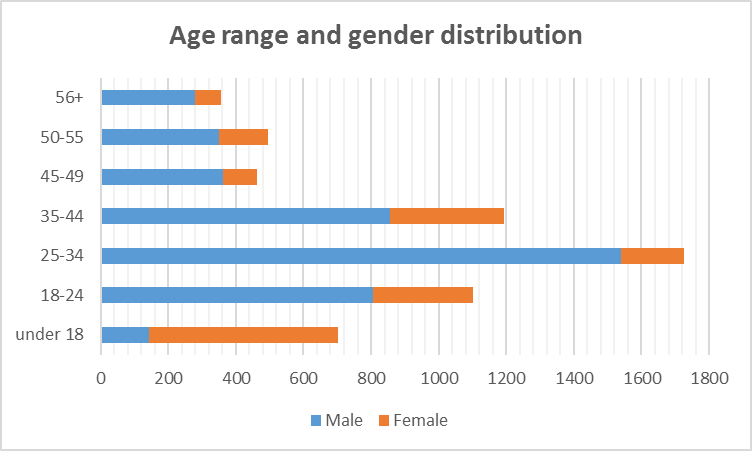
\includegraphics[width=\columnwidth]{images/agerange_gender.png}
\caption{"Male" and "25" have higher densities in users data}
\label{fig:agerangegender}
\end{figure}

\section{Proposed Method}

For this task, we worked on two sets of approaches: Early-fusion (parallelized design) and Late-fusion (monolithic design). For the early-fusion approach, we boosted item-based collaborative filtering using content-based movies similarity, and user-based collaborative filtering using content-based users similarity.  Finally, we boosted matrix factorization approach by trying two different approaches, namely SVD++ and gSVD++.
For the late fusion approach, we combined the results of multiple recommendation systems using a regression model.

\subsection{Early-Fusion Approach}

This approach adapts our prior collaborative filtering and content based algorithms to deal with modified hybrid input data. This data contains combinations and/or augmentations of data from multiple different sources.

\subsubsection{Item-based Collaborative Filtering (IBCF)}

This approach measures the similarity between items to recommend similar items for a user or predict how would he/she rate an item. When users rate an item, its similar items are picked from the existing system model and added to user's recommendations. This approach is usually preferred over other memory-based approaches (user-based) when the system has more users than items as it leads to a more stable rating distribution.

Figure (\ref{fig:ibcf_approach}) shows the basic steps of IBCF approach to predict how a user would rate an item. First a model is built by finding the similarity between all pairs of items. Then, the most similar $ k $ items which have been already rated by the user are selected to compute the predicted rating of that user for the item. This computed rating is the average rating of all selected items rated by that user.

The similarity between two items is calculated using a weighted sum scheme that combines the ratings-based similarity that uses previous users' ratings and the content-based similarity that uses the crawled information from on-line movie sources. The following equation shows how the similarity between two movies is calculated:
\begin{equation}
sim(x, y) = (1 - \alpha) \times sim_{r}(x, y) + (\alpha) \times sim_{a}(x, y)
\end{equation}
Where:

$ sim_{r} $ is the ratings-based similarity between the movies (m1, m2)

$ sim_{a} $ is the content-based similarity between the movies (m1, m2)

$ \alpha $  is a weighting factor, in practice this factor performed best when set to (1.0), which means using only the content-based similarity

The crawled movie attributes were divided into seven categories as follows:
\begin{itemize}
	\item Year: contains the release year of the movie
	\item Rating: contains all crawled ratings of the movie (Tomato Meter, IMDB Rating, Tomato User Rating, …)
	\item Genres: contains genres of the movie
	\item Stakeholders: contains all main players in the movie production (writers, actors, directors and production companies)
	\item Description: contains all text descriptions crawled from the different sources
	\item Other: contains any other important features (awards, …)
\end{itemize}
For each category, a specific similarity measure is used. Then, the similarity between two movies is calculated as a weighted sum of the similarities between their categorized attributes. The measures for each attribute category were discussed in more detail in task 2.

\begin{figure}
	\centering
	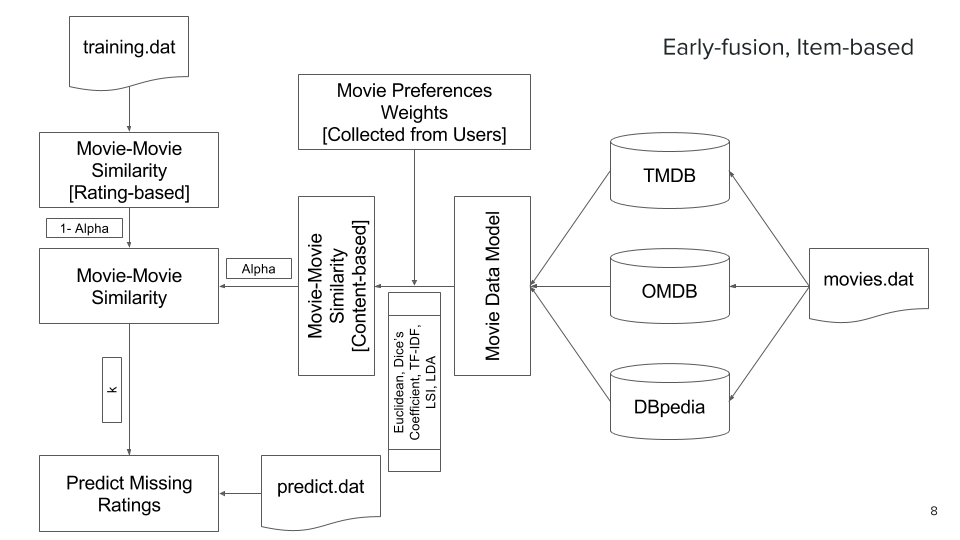
\includegraphics[width=\columnwidth]{images/ibcf_approach.png}
	\caption{Item-based collaborative filtering approach}
	\label{fig:ibcf_approach}
\end{figure}

\subsubsection{User-based Collaborative Filtering (UBCF)}

This approach measures the similarity between users to recommend new items for a user or predict how would he/she rate an item based on the ratings of other similar users. This approach is widely used and has good recommendation results but it does not scale with the number of users when it goes very high.

Figure (\ref{fig:ubcf_approach}) shows the basic steps of UBCF approach to predict how a user would rate an item. First a model is built by finding the similarity between all pairs of current users. Then, the most similar $ k $ users which have already rated the item are selected to compute the predicted rating of that user for the item. This computed rating is the average rating of all selected users.

The similarity between two users is calculated using a weighted sum scheme similar to the one used for calculating the similarity between two movies. This scheme also combines ratings-based similarity and content-based similarity that uses the users information provided in the third file (the users set).

Content-based similarity between two users is calculated as a weighted sum of the individual similarities between their attributes. Age and zip-code similarities were measured using the Euclidean distance. Gender and job similarities were measured using a binary scheme, where two values are either similar (when they match exactly) or not similar (when they differ).

The weights for combining individual similarities into the final content-based similarity between two users were set manually due to the lack of evaluation time and resources.

\begin{figure}
	\centering
	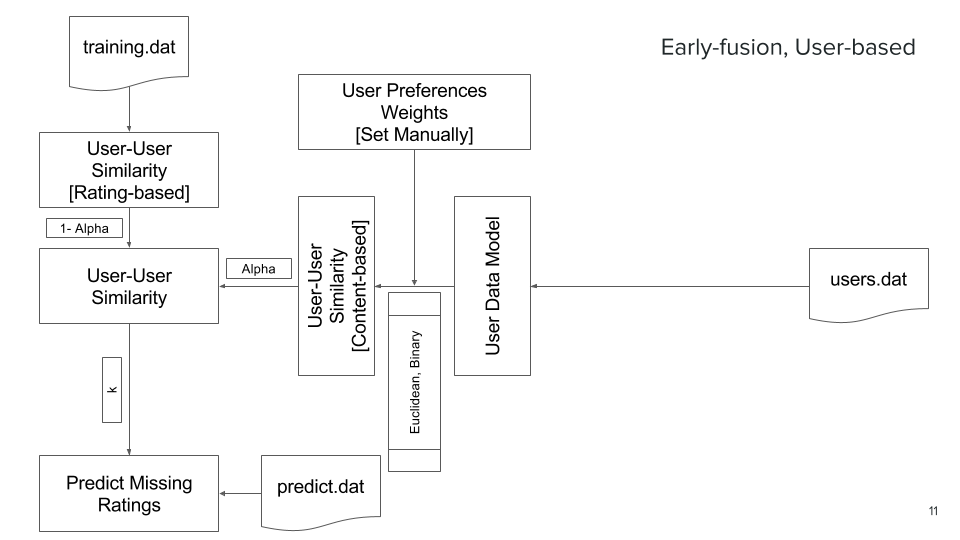
\includegraphics[width=\columnwidth]{images/ubcf_approach.png}
	\caption{User-based collaborative filtering approach}
	\label{fig:ubcf_approach}
\end{figure}

\subsubsection{Matrix Factorization}

This approach estimates hidden (meta) parameters from user ratings to try describing them in a higher dimensional space (compared to the original dimensions of user and item). These parameters are called latent factors and they are not necessarily interpretable. This approach maps the two dimensions into the new latent ones and try to minimize the reconstruction error using multiple approaches like Singular Value Decomposition (SVD) or Gradient Descent.

We tried to evaluate two extensions of matrix factorization.

\textbf{\emph{Singular Value Decomposition++ (SVD++) }}
\newline

This approach improves the accuracy of SVD using explicit and implicit feedback from users. The preferences of a user are represented using a combination of these explicit and implicit feedbacks.

In out case, the explicit feedback of a user is based on the movie ratings he/she made and the implicit feedback is based on the movies a user rated, without consideration of the rating values.

\textbf{\emph{gSingular Value Decomposition++ (gSVD++) }}

This approach enriches implicit and explicit feedbacks from SVD++ using meta-information about the items. This information could be aggregated from external sources as introduced earlier (genres, actors, ...).

\subsection{Late-Fusion Approach}

This approach aggregates the outputs of multiple recommendation systems into one final recommendation. The aggregation could be using weighting or voting schemes. In the weighting scheme, the results of all individual recommendation systems are combined, so the final result may differ from all individual results. In the voting scheme, each individual recommendation system votes for a result (for example, increment its occurrences by one). The final recommendation is the individual recommendations with the highest votes.

Figure (\ref{fig:late_fusion_approach}) shows the basic steps of late-fusion approach. Five different recommendation systems were aggregated using a weighting scheme. To set the weights, we used a K-Nearest-Neighbor regression model. The outputs of these five recommendation systems are merged together in a file where each column represents the predicted rating for each individual approach. One column contains the actual ratings from the test set. Subsequently these outputs are used as input to train the regression model and determine the optimal weights to minimize the introduced error. Using an optimized weighting scheme, the final output is the submitted rating.

The five recommendation systems which were aggregated are:
\begin{itemize}
	\item Item-based collaborative filtering
	\item User-based collaborative filtering
	\item Matrix factorization
	\item Content-based collaborative filtering (with movies information as the content)
	\item Content-based collaborative filtering (with users information as the content)
\end{itemize}

\begin{figure}
	\centering
	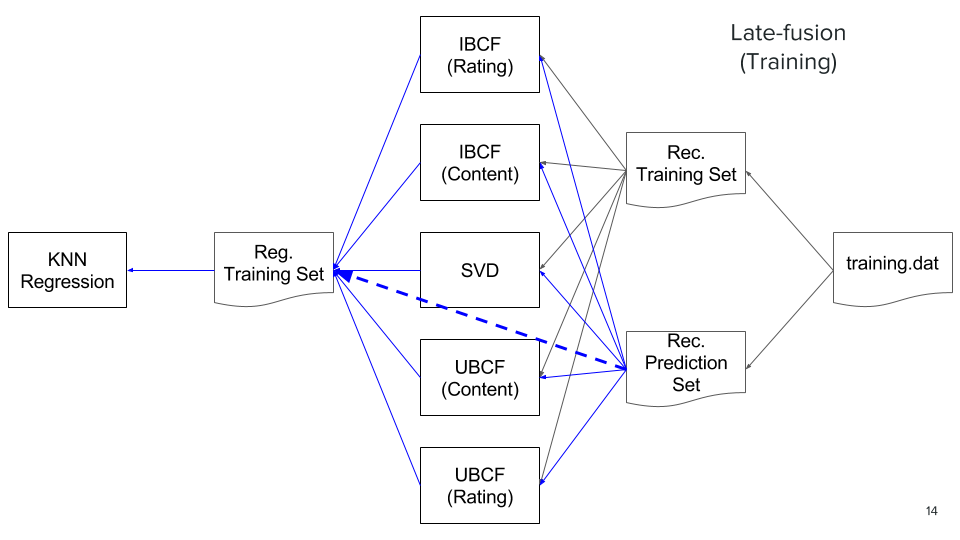
\includegraphics[width=\columnwidth]{images/late_fusion_approach.png}
	\caption{Late-fusion approach}
	\label{fig:late_fusion_approach}
\end{figure}

\section{Experimental Setup}

As the final predictions of the task are evaluated using Root Mean Square Error (RMSE), we used this measure to evaluate our models. To make sure that the evaluation is not biased, we used 10-fold cross validation on the provided ''training.dat'' file as the true ratings are provided. Using cross-validation will ensure that no triples (user, item, rating) are used in both training (building) and evaluating the model.

To compare results of the different evaluated approaches, we introduced a simple mean-user-ratings approach as a baseline. This approach simply predicts the missing rating of a user for an item by averaging all his previous ratings.

\subsection{Content-based Similarities}
Tuning all the weights automatically for content-based similarity measures (for movies and users) is not feasible as each single evaluation takes from (10-60) hours. We set these weights manually using a simple voting approach. Multiple persons were asked to rank their preferences and the average rankings were used to compute the weights (more details are available in task 2). Tables (\ref{tab:movie_weights}, \ref{tab:user_weights}) show the weights for each set of attributes for movies and users respectively.

\begin{table}[]
\centering
\begin{tabular}{|l|c|c|}
\hline
\textbf{Attribute} & \textbf{Weight} \\ \hline
Year             & 5               \\ \hline
Rating             & 6               \\ \hline
Genres             & 7               \\ \hline
Actors             & 5               \\ \hline
Production Companies             & 3               \\ \hline
Directors             & 4               \\ \hline
Writers             & 4               \\ \hline
Description             & 6               \\ \hline
Other             & 2               \\ \hline
\end{tabular}
\caption{Weights of movie features}
\label{tab:movie_weights}
\end{table}

\begin{table}[]
	\centering
	\begin{tabular}{|l|c|c|}
		\hline
		\textbf{Attribute} & \textbf{Weight} \\ \hline
		Gender             & 5               \\ \hline
		Age             & 4               \\ \hline
		Job             & 3               \\ \hline
		Zip-code             & 2               \\ \hline
	\end{tabular}
	\caption{Weights of user features}
	\label{tab:user_weights}
\end{table}

\subsection{k-Nearest-Neighbors Regression}
As input for the parallelized hybridization, the predictions from different individuals approaches, which were listed earlier, were used. The were run again on the latest training and test data with their optimized setup which yielded the best results in the prior tasks. Due to performance and time reasons the individual computed predictions were stored as model files for later re-usage. Tuning the setup for the late fusion approach relies on a k-Nearest-Neighbor regression model to predict optimal target weights for the final weighted hybrid run. To build a regression model the output from different individual approaches as well as the actual rating were split into a training and test set and then fitted into the k-Nearest-Neighbor regression model. Using cross validation, within each fold the regressor predicts the values for the test set and computes the RMSE between result and actual rating. We tuned the "number of neighbors" parameter to get the best RMSE. Table \ref{tab:regrRMSE} shows a part of the tried ranges. Based on the collected data from the classifier training the values, which yielded the best RMSE as evaluation criteria, were chosen for the final predictions.
\begin{table}
\centering	
	\begin{tabular}{|c|c|}
	\hline
	\textbf{Number of neighbors} & \textbf{RMSE} \\ \hline
	\textbf{nn = 1}  & 1.2571         \\ \hline
	\textbf{nn = 5} & 0.9747         \\ \hline
	\textbf{nn = 10} & 0.9334         \\ \hline
	\textbf{nn = 20} & 0.9121         \\ \hline
	\textbf{nn = 40} & 0.9015         \\ \hline
	\textbf{nn = 80} & 0.8961         \\ \hline
	\textbf{nn = 160} & 0.8934         \\ \hline
	\textbf{nn = 320} & 0.8923         \\ \hline
	\textbf{nn = 430} & \textbf{0.8921}         \\ \hline
	\textbf{nn = 750} & 0.8921         \\ \hline
	\textbf{nn = 1280} & 0.8922         \\ \hline
	\end{tabular}
	\caption{RMSE results for the regression model}
	\label{tab:regrRMSE}
\end{table}

\subsection{SVD++ \& gSVD++}
For SVD++, we used the parameters from \cite{Koren:2009} which were used for a similar task with the Netflix dataset, assuming that Netflix's dataset is similar to the one we are provided with. Using these parameters, we evaluated different number of latent factors.
\begin{itemize}
\item Regularization = 0.015
\item Bias regularization = 0.33
\item Learn rate = 0.001
\item Bias learn rate = 0.7
\item Learn rate decay = 1
\end{itemize}

gSVD++ is based on SVD++. Therefore, we configured it using the same parameters mentioned above. We also used the number of factors which gave the best results for SVD++. Meta-information about the movies was provided to gSVD++ algorithm using created lists which maps our crawled movie attributes to the defined categories of attributes for gSVD++.
\emph{We were not able to get results for this approach, due to lack of resources (memory resources). When our created lists for the movies and their associated crawled attributes reached a certain size, the script stopped with an out of memory exception.}

\section{Results}

Table (\ref{tab:eval_00}) shows the evaluation results from the first task for IBCF using the cosine similarity measure. We can see that the best performance was at $ k = 1 $

\begin{table}[]
\centering
\begin{tabular}{|c|c|}
\hline
                & \textbf{IBCF} \\ \hline
\textbf{k = 1}  & 1.037         \\ \hline
\textbf{k = 10} & 1.115         \\ \hline
\textbf{k = 15} & 1.123         \\ \hline
\textbf{k = 20} & 1.129         \\ \hline
\textbf{k = 30} & 1.134         \\ \hline
\textbf{k = 40} & 1.135         \\ \hline
\end{tabular}
\caption{First Task Results for IBCF}
\label{tab:eval_00}
\end{table}

Table (\ref{tab:eval_01}) and Figure (\ref{fig:eval_01}) show the results of the first evaluation set along with the baseline. From them, we can see that all the tested text similarity mesures (TF-IDF, LSI, LDA) performed very closely with LSI having the best performance at $ k = 15 $.

\begin{table}[]
\centering
\begin{tabular}{|c|c|c|c|c|}
\hline
                & \textbf{Baseline} & \textbf{TF-IDF} & \textbf{LSI}   & \textbf{LDA} \\ \hline
\textbf{k = 1}  & 1.036             & 1.224           & 1.222          & 1.221            \\ \hline
\textbf{k = 10} & 1.036             & 0.948           & 0.946          & 0.947            \\ \hline
\textbf{k = 15} & 1.036             & 0.952           & \textbf{0.944} & 0.947            \\ \hline
\textbf{k = 20} & 1.036             & 0.946           & 0.947          & 0.947            \\ \hline
\textbf{k = 30} & 1.036             & 0.951           & 0.949          & 0.947            \\ \hline
\textbf{k = 40} & 1.036             & 0.954           & 0.955          & 0.947            \\ \hline
\end{tabular}
\caption{First Evaluation Set - $ \alpha = 1.0 $}
\label{tab:eval_01}
\end{table}

\begin{figure}
\centering
%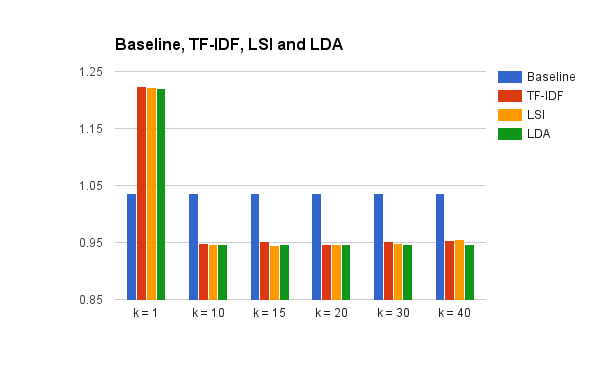
\includegraphics[width=\columnwidth]{images/evaluations.png}
\caption{First Evaluation Set - $ \alpha = 1.0 $}
\label{fig:eval_01}
\end{figure}

Table (\ref{tab:eval_02}) shows the results of the second evaluation set. In this set, we fixed $ k = 10 $ and run using only LSI model as it has the best performance in the first evaluation set. $ k = 10 $ is fixed between the best values of $ k $ in IBCF in the first and second task. It is closer to the best $ k $ in the second task as it's performance is relatively better.

\begin{table}[]
\centering
\begin{tabular}{|c|c|}
\hline
                     & \textbf{LSI} \\ \hline
\textbf{alpha = 0.0} & 1.115        \\ \hline
\textbf{alpha = 0.2} & 0.947        \\ \hline
\textbf{alpha = 0.4} & 0.948        \\ \hline
\textbf{alpha = 0.6} & 0.949        \\ \hline
\textbf{alpha = 0.8} & 0.949        \\ \hline
\textbf{alpha = 1.0} & 0.946        \\ \hline

\end{tabular}
\caption{Second Evaluation Set - $ k = 10 $}
\label{tab:eval_02}
\end{table}

Table (\ref{tab:svd_02}) shows the evaluation results for the SVD++ for different factors. We can see that the best performance was with the use of ??? factors.

\begin{table}[]
\centering
\begin{tabular}{|c|c|}
\hline
                     & \textbf{SVD++} \\ \hline
\textbf{number of factors = 10} & 0,8960        \\ \hline
\textbf{number of factors  = 50} & ---        \\ \hline
\textbf{number of factors  = 100} & ---        \\ \hline
\textbf{number of factors  = 200} & ---        \\ \hline

\end{tabular}
\caption{SVD++ for different factors}
\label{tab:svd_02}
\end{table}

\section{Conclusions}

TF-IDF, LSI and LDA were so close in their performance having LSI as the best performer in combination with $ k = 10 $. The evaluated text models didn't affect the final results much as there are other attributes affecting the similarity between two movies. Tuning all parameters for these attributes needs much more resources than we have. Although the results were close, we preferred to go with best performer to predict the final missing ratings in the file ''predict.dat''


% The following two commands are all you need in the
% initial runs of your .tex file to
% produce the bibliography for the citations in your paper.
\bibliographystyle{abbrv}
\bibliography{refs}  % refs.bib is the name of the Bibliography in this case
% You must have a proper ".bib" file
%  and remember to run:
% latex bibtex latex latex
% to resolve all references

\end{document}
